\chapter{Repositórios}\label{Repositórios}\lhead{\leftmark}

A arquitetura descentralizada do Baobáxia é baseada em repositórios
\emph{git} e \emph{git-annex}.

Um elemento importante para o acervo multimídia são as operações de
sincronização. As ferramentas baseadas no \emph{git} herdam a sua
natureza descentralizada e a capacidade de comunicar de forma
transparente usando vários protocolos. Em particular é interessante a
possibilidade de executar sincronizações com sistemas de armazenamento
massivo, característica essencial na fase de criação de um novo nó,
onde a primeira sincronização via rede poderia levar dias. As
transferências contudo, no caso do \emph{git-annex}, são executadas
através do protocolo \emph{rsync}\footnote{\emph{rsync} é um Software
  Livre para a transfêrencia rápida e incremental de arquivos
  disponível no \url{http://rsync.samba.org/}.}, que gerencia
eventuais interrupções, evitando retransmissões onerosas.


\subsection{Git}\label{sec:GIT}
Git é um sistema multiplataforma para o controle de versão
distribuído, projetado para ser rápido e usável mesmo em grande
projetos.

As características principais incluem:
\begin{itemize}
\item é totalmente distribuído e cada clone de um repositório contem o
  histórico inteiro das versões e no qual podem ser efetuadas
  operações independentemente de conexões de rede o de servidores
  centrais. As mudanças podem ser copiadas entre um clone e o outro e
  são mantidos em \emph{branch} (ramos) diferentes, facilitando as
  operações de \emph{merge} (fusão). Os repositórios são facilmente
  acessíveis através do eficiente protocolo do Git, que além de
  suportar HTTP, pode funcionar junto com SSH, para obter conexões
  seguras e um sistema de autenticação solido e bem comum.
\item suporta o \emph{branching} (ramificação), e o \emph{merging}
  (fusão), de maneira rápida e conveniente, incluindo uma serie de
  ferramentas para visualizar e navegar o histórico não linear das
  versões.
\item é muito rápido e escala mesmo em projetos muito grandes e com
  muitas mudanças, graças a um eficiente sistema de empacotamento e
  memorização do histórico (é considerado o mais eficiente entre os
  sistemas atualmente disponíveis).
\item associa um nome de versão, para cada \emph{commit}, que é função
  do histórico inteiro, por isso, uma vez publicada uma versão, não é
  possível alterar as velhas sem ser notado. As versões podem também
  ser etiquetadas e assinadas digitalmente com GPG.
\end{itemize}

Git é um sistema completo que, em bom estilo Unix, é organizado em
programas e comandos independentes, pensados para ser facilmente
usáveis, seja automaticamente através de \emph{scripting} seja de
maneira interativa pelo usuário final. Git é, então, uma base solida
para o desenvolvimento de aplicações orientadas a sincronização, a
portabilidade e a gestão autônoma e descentralizada. 

\subsection{git-annex}\label{git-annex}
\emph{git-annex}\footnote{\emph{git-annex} é um programa que estende
  as funcionalidades do \emph{git} em gerir arquivos de grande tamanho
disponível no \url{http://git-annex.branchable.com}.} permite a
gestão de arquivos com \emph{git}, sem a necessidade de adicionar os
arquivos dentro \emph{git}. Mesmo se pode parecer paradoxal, é útil
quando se trabalha com arquivos muito grandes que \emph{git}
atualmente não gerencia facilmente por limitações devidas a memoria,
tempo ou espaço no disco.

Mesmo sem manter o histórico das mudanças do conteúdo do arquivo, ter
a possibilidade de gerenciar arquivos com \emph{git}, de movê-los, e
exclui-los, numa árvore de pasta versionada, com uso de
\emph{branches} e de clones distribuídos, são todos bons motivos para
usar \emph{git}. E os arquivos anexos (por isso o nome
\emph{git-annex}) podem coexistir no mesmo repositório \emph{git} com
os arquivos regularmente versionados. 

\emph{git-annex} transforma os arquivos anexos em \emph{link}
simbólicos, que são normalmente versionados por \emph{git}. 

O conteúdo dos arquivos é mantido por \emph{git-annex} em um acervo
chave/valor distribuído que corresponde aos clones de um dado
repositório \emph{git}. Praticamente \emph{git-annex} memoriza o
conteúdo do arquivo em uma subpasta de \verb|.git/annex/|.

A primeira vez que um arquivo é adicionado no \emph{git-annex}, é
calculada uma chave, normalmente fazendo um \emph{hash} do seu
conteúdo. \emph{git-annex} todavia suporta vários \emph{backend} que
podem produzir diferentes tipos de chaves. O arquivo que é adicionado
no \emph{git} nada mais é que um \emph{link} simbólico para a chave
memorizada no \verb|.git/annex/|. Se o conteúdo do arquivo for
modificado, é gerada uma outra chave, e o \emph{link} é alterado. 

O conteúdo do arquivo pode ser transferido de um repositório para
outro por \emph{git-annex}, que além de manter controle de quem mantem
o que, permite criar um mapa das copias disponíveis e impor um número
mínimo de cópias. Essas informações são mantidas em um \emph{branch}
separado, chamado ``\emph{git-annex}'', e as operações de
sincronização, são simplesmente \emph{push} e \emph{pull} entre os
vários clones dos repositórios.

\emph{git-annex} suporta:
\begin{itemize}
\item localização das cópias (\emph{location tracking})
\item download seletivo dos conteúdos 
\item gestão da confiança dos repositórios
\item gestão do número minimo de cópias
\item vários \emph{backend} para as chaves (SHA\footnote{Secure Hash
    Algoritm, (SHA), é um algoritmo usado em sistemas chave/valor onde
    as chaves são calculadas através de uma função criptográfica dos
    valores.}, WORM\footnote{O algoritmo WORM identifica os arquivos
    em base ao nome, dimensão e data de alteração.})
\item vários \emph{backend} para os conteúdos/valores
  (BUP\footnote{BUP é um sistema para \emph{backup} a alta eficiência
    disponível no: \url{https://github.com/apenwarr/bup}.}, rsync,
  web, S3\footnote{Amazon Simple Storage Service, (S3) é uma
    infraestrutura para a memorização dos dados totalmente redundante,
    disponível no: \url{aws.amazon.com/}.})
\end{itemize}

\section{Gestão de repositórios multiplos}
A arquitetura baseadas em repositórios se adapta ao contexto de
``redes federadas'' onde para cada ``Rede'' corresponde um
repositório. A solução proposta no Baobáxia inclui já a possibilidade
de cadastrar e gerenciar varias redes. A associação rede/repositório
permite a escalabilidade da arquitetura e uma gestão diferenciada dos
conteúdos. Cada mucua pode se associar a diferentes redes, por
exemplo, Rede Mocambos, Estaçoes Digitais, etc.

\begin{figure}[htbp]
  \centering
  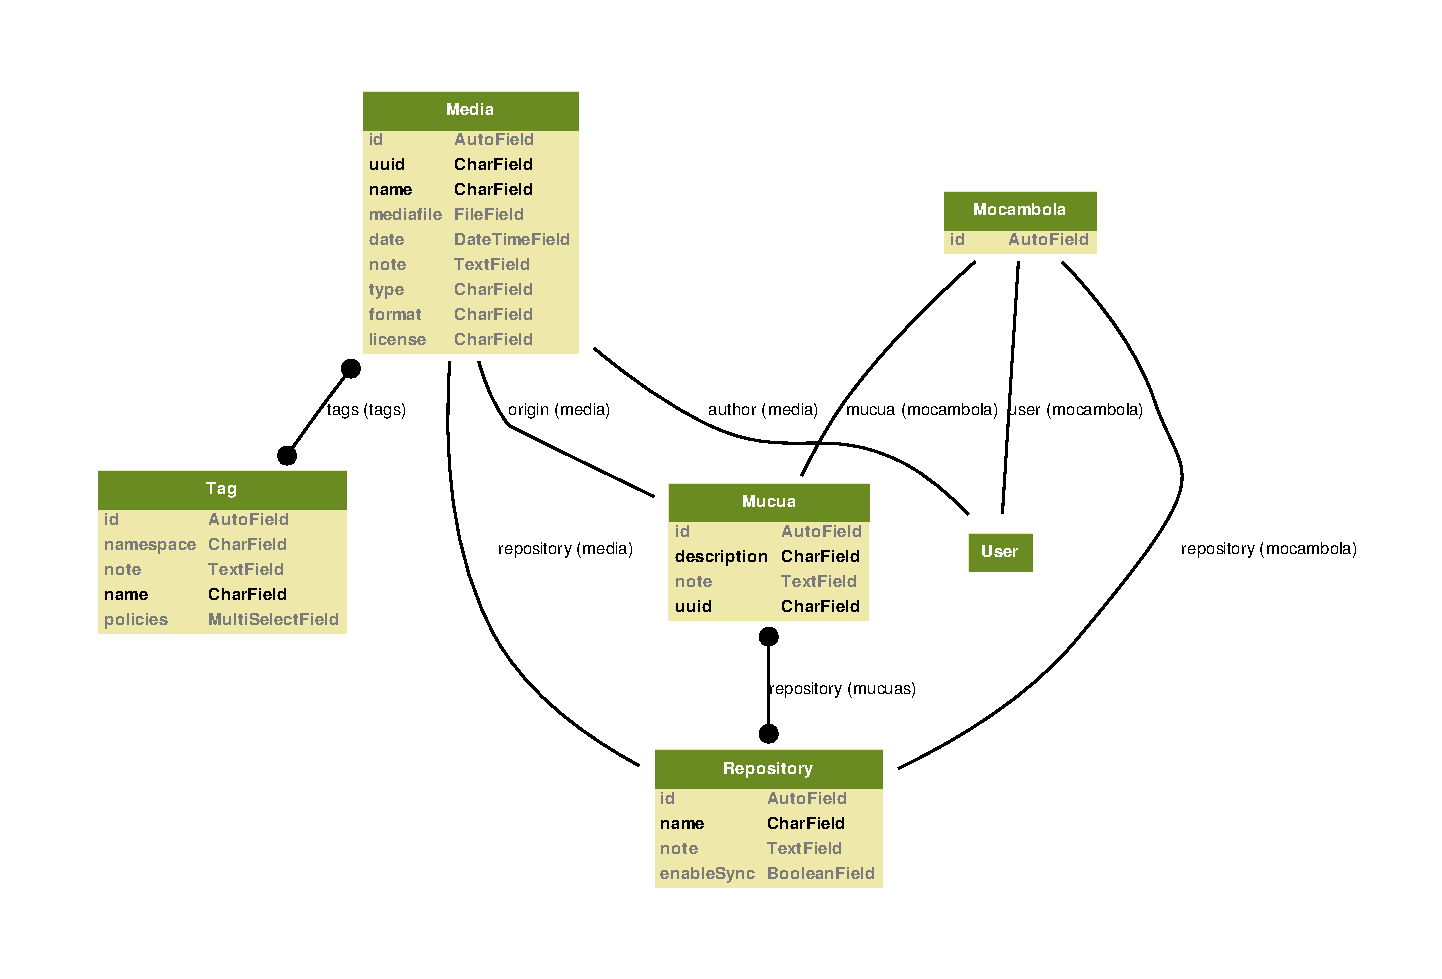
\includegraphics[width=\textwidth]{./Fig/Auto_UML_Diagram.pdf}
  \rule{35em}{0.5pt}
  \caption[Diagrama UML do BBX]{Diagrama UML do BBX}
  \label{fig:SchemaServer_ReteMocambos}
\end{figure}

\subsection{API e rotas}
A API REST proposta prevê a gestão de repositórios multiplos em
diferentes mucuas, usando o padrão de endereços:
$$ /repositorio/mucua/ $$ 

Por exemplo, para acessar um ``media'' (uuid
aa9f9019-e4f2-4040-bc46-c2e15b66bebc) publicado na ``Rede Mocambos'', na
mucua ``Dandara'' o endereço é:
$$ /mocambos/dandara/media/aa9f9019-e4f2-4040-bc46-c2e15b66bebc $$

ou no caso da ``Estaçao Digital'' na ``Samambaia'' seria:
$$ /fbb/samambaia/media/aa9f9019-e4f2-4040-bc46-c2e15b66bebc $$

O detalhamento da API e das rotas será definido em capitulo especifico. % REF.

\subsection{Autenticação}
O Baobáxia pode gerenciar dados de varias redes/organizações e
portanto precisa diferenciar os usuários por Rede e Mucua\footnote{A
  mucua de alguma forma identifica uma comunidade}. No caso as
credenciais dos usuários são mantidas em arquivos versionados pelo git
nos repositórios correspondentes.

Para manter compatibilidade com outras aplicações do django mantivemos
o User padrão do django usando somente o campo username para codificar
as informarções necessárias.

Um mocambola\footnote{Usuário} é definido por nome, mucua e
repositorio no padrão:
$$ nome@mucua.repositorio.tld $$ .

O django é muito flexivel e suporta diferentes sistemas de
autenticação, com a possibilidade de definir seu proprio backend
personalizado.

O backend de autenticação personalizado, ``FileBackend'' se encontra
em \emph{bbx/auth.py}.

No BBX, os usuários são serializados em formato \emph{json} e
armazenados seguindo o seguinte padrão de localização:
$$ /repositorio/mucua/mocambolas/usuario.json $$

Por exemplo, no caso do mocambola ``zumbi'' da Casa de Cultura
Tainã cuja mucua se chama ``dandara'':
$$ zumbi@dandara.mocambos.net $$
$$ /mocambos/dandara/mocambolas/zumbi@dandara.mocambos.net $$

Notar que o repositório não inclui a extensão de dominio de primeiro
nível, no caso do exemplo ``.net'', que permanece no username do
mocambola.



